\subsubsection{Polymethylmethacrylat}
\label{subsec:pofpmma}

Polymethylmethacrylat (PMMA) wurde erstmals 1928 von Otto Röhm hergestellt. Fünf
Jahre später wurde PMMA unter dem Namen
Plexiglas\textsuperscript{\textregistered} vermarktet. Aufgrund der hohen
optischen Durchlässigkeit und des geringen Gewichts eignet sich PMMA für den
Einsatz in der Automobilindustrie. Diese Eigenschaften sind ebenfalls ein
Grund für die Verwendung von PMMA in polymer optischen Fasern. \cite{pofwuppmma}

\paragraph{Polymerisation von Polymethylmethacrylat} Die Synthese von PMMA
erfolgt mittels einer radikalischen Polymerisation. Dabei wird zu dem Monomer
Methylmethacrylat (MMA) ein Radikalbildner gegeben. Der Radikalbildner zerfällt
durch Licht- / Wärmezufuhr in Radikale. Diese lagern sich an die
C-C-Doppelbindung der Monomere an. Dadurch wird die Doppelbindung des MMAs
aufgespalten und das aktive Zentrum weitergegeben. Dieser Vorgang erzeugt wieder
ein Radikal, welches ebenfalls ein Methylmethacrylat angreift. Dadurch wächst
die Monomerkette zu einem Polymer an. Der Abbruch des Kettenwachstums kann
entweder durch einen Zusammenschluss mit einem weiteren Radikal oder durch eine
Disproportionierung geschehen. Beide Reaktionen haben eine Sättigung des aktiven
Zentrums zur Folge. \autoref{rec:pmma} fasst den Reaktionsablauf zusammen und
zeigt, dass es sich bei Polymethylmethacrylat um ein lineares Makromolekül also
um einen Thermoplasten handelt.

\begin{figure}[H]
    \begin{center}
        \footnotesize
        \setatomsep{1.7em}

        \chemnameinit{\chemfig{-[@{op,0.5}]CH_2-C(-[2]CH_3)(-[6]C(=[:-150]\lewis{36,O})(-[:-30]\lewis{57,O}-[:30]CH_3))-[@{cl,0.9},3.1pt]}}

        \chemname{\chemfig{R-R}}{\\\\Radikalbildner}
        \chemsign{+ $\scriptstyle n$}
        \chemname{\chemfig{H_2C=C(-[:60]CH_3)(-[:-60]C(=[:-120]\lewis{46,O})(-\lewis{26,O}-CH_3))}}{\\\\Methylmethacrylat}
        \chemrel{->}
        \chemname{\chemfig{-[@{op,0.5}]CH_2-C(-[2]CH_3)(-[6]C(=[:-150]\lewis{36,O})(-[:-30]\lewis{57,O}-[:30]CH_3))-[@{cl,0.9},3.1pt]}}{\\\\Polymethylmethacrylat}
        \makebraces[20pt,35pt]{n}{op}{cl}

        \caption{radikalische Polymerisation von Polymethylmethacrylat}
        \label{rec:pmma}
    \end{center}
\end{figure}


\paragraph{Versuch: Herstellung von PMMA}

Material:
\begin{itemize*}
    \item Heizplatte, Reagenzgläser, Thermometer, Wasserbad, Spatel, Waage, Stativ
    \item Chemikalien: Methylmethacrylat (MMA; Sicherheitshinweis: CAS Nr. 80-62-1 (\autoref{fig:flamme}, \autoref{fig:ausrufezeichen})), Azodiisobutyronitril (AIBN; Sicherheitshinweis: CAS Nr. 80-62-1 (\autoref{fig:flamme}, \autoref{fig:ausrufezeichen})), Dibenzoylperoxid (BPO; Sicherheitshinweis: CAS Nr. 80-62-1 (\autoref{fig:flamme}, \autoref{fig:ausrufezeichen}, \autoref{fig:bombe}))
\end{itemize*}

\begin{figure}[h]
    \begin{center}
        \begin{minipage}[t]{0.25\textwidth}
            \begin{center}
                \includegraphics[height=0.1\textheight]{Bilder/Optische_Wellenleiter_Die_Polymer_Optische_Faser/Material_Polycarbonat/flamme.png}
                \caption[entzündlicher Stoff \newline \url{https://de.wikipedia.org/wiki/Datei:GHS-pictogram-flamme.svg} (zuletzt aufgerufen am 11.10.2015)]{entzündlicher Stoff}
                \label{fig:flamme}
            \end{center}
        \end{minipage}
        \hspace{0.025\textwidth}
        \begin{minipage}[t]{0.25\textwidth}
            \begin{center}
                \includegraphics[height=0.1\textheight]{Bilder/Optische_Wellenleiter_Die_Polymer_Optische_Faser/Material_Polycarbonat/ausrufezeichnen.png}
                \caption[reizender Stoff \newline \url{https://de.wikipedia.org/wiki/Datei:GHS-pictogram-exclam.svg} (zuletzt aufgerufen am 11.10.2015)]{reizender Stoff}
                \label{fig:ausrufezeichen}
            \end{center}
        \end{minipage}
        \hspace{0.025\textwidth}
        \begin{minipage}[t]{0.25\textwidth}
            \begin{center}
                \includegraphics[height=0.1\textheight]{Bilder/Optische_Wellenleiter_Die_Polymer_Optische_Faser/Material_Polycarbonat/bombe.png}
                \caption[explosiver Stoff \newline \url{https://de.wikipedia.org/wiki/Datei:GHS-pictogram-explos.svg} (zuletzt aufgerufen am 11.10.2015)]{explosiver Stoff}
                \label{fig:bombe}
            \end{center}
        \end{minipage}
    \end{center}
\end{figure}

Schutzvorkehrungen:
\begin{itemize}
    \item Abzug, Schutzkleidung, Handschuhe, Schutzbrille
\end{itemize}

Versuchsablauf:
\begin{enumerate*}
    \item Das Wasserbad wird unter dem Abzug auf ca. 70°C erhitzt.
    \item In einem Reagenzglas werden 5 ml MMA mit 50 mg BPO / AIBN vermischt.
    \item Das Reagenzglas wird im Wasserbad erhitzt (siehe \autoref{fig:mmawasserbad}).
    \item Sobald der Inhalt des Reagenzglases zähflüssig ist, wird das Reagenzglas aus dem Wasserbad genommen.
    \item Sobald die Polymerisation abgeschlossen ist, wird das Reagenzglas zerschlagen und das PMMA kann entnommen werden.
\end{enumerate*}

\begin{figure}[h]
    \begin{center}
        \begin{minipage}[t]{0.4\textwidth}
            \begin{center}
                \includegraphics[height=0.1\textheight]{Bilder/Optische_Wellenleiter_Die_Polymer_Optische_Faser/Material_Polycarbonat/mmawasserbad.png}
                \caption[Versuchsaufbau]{Versuchsaufbau}
                \label{fig:mmawasserbad}
            \end{center}
        \end{minipage}
        \hspace{0.025\textwidth}
        \begin{minipage}[t]{0.4\textwidth}
            \begin{center}
                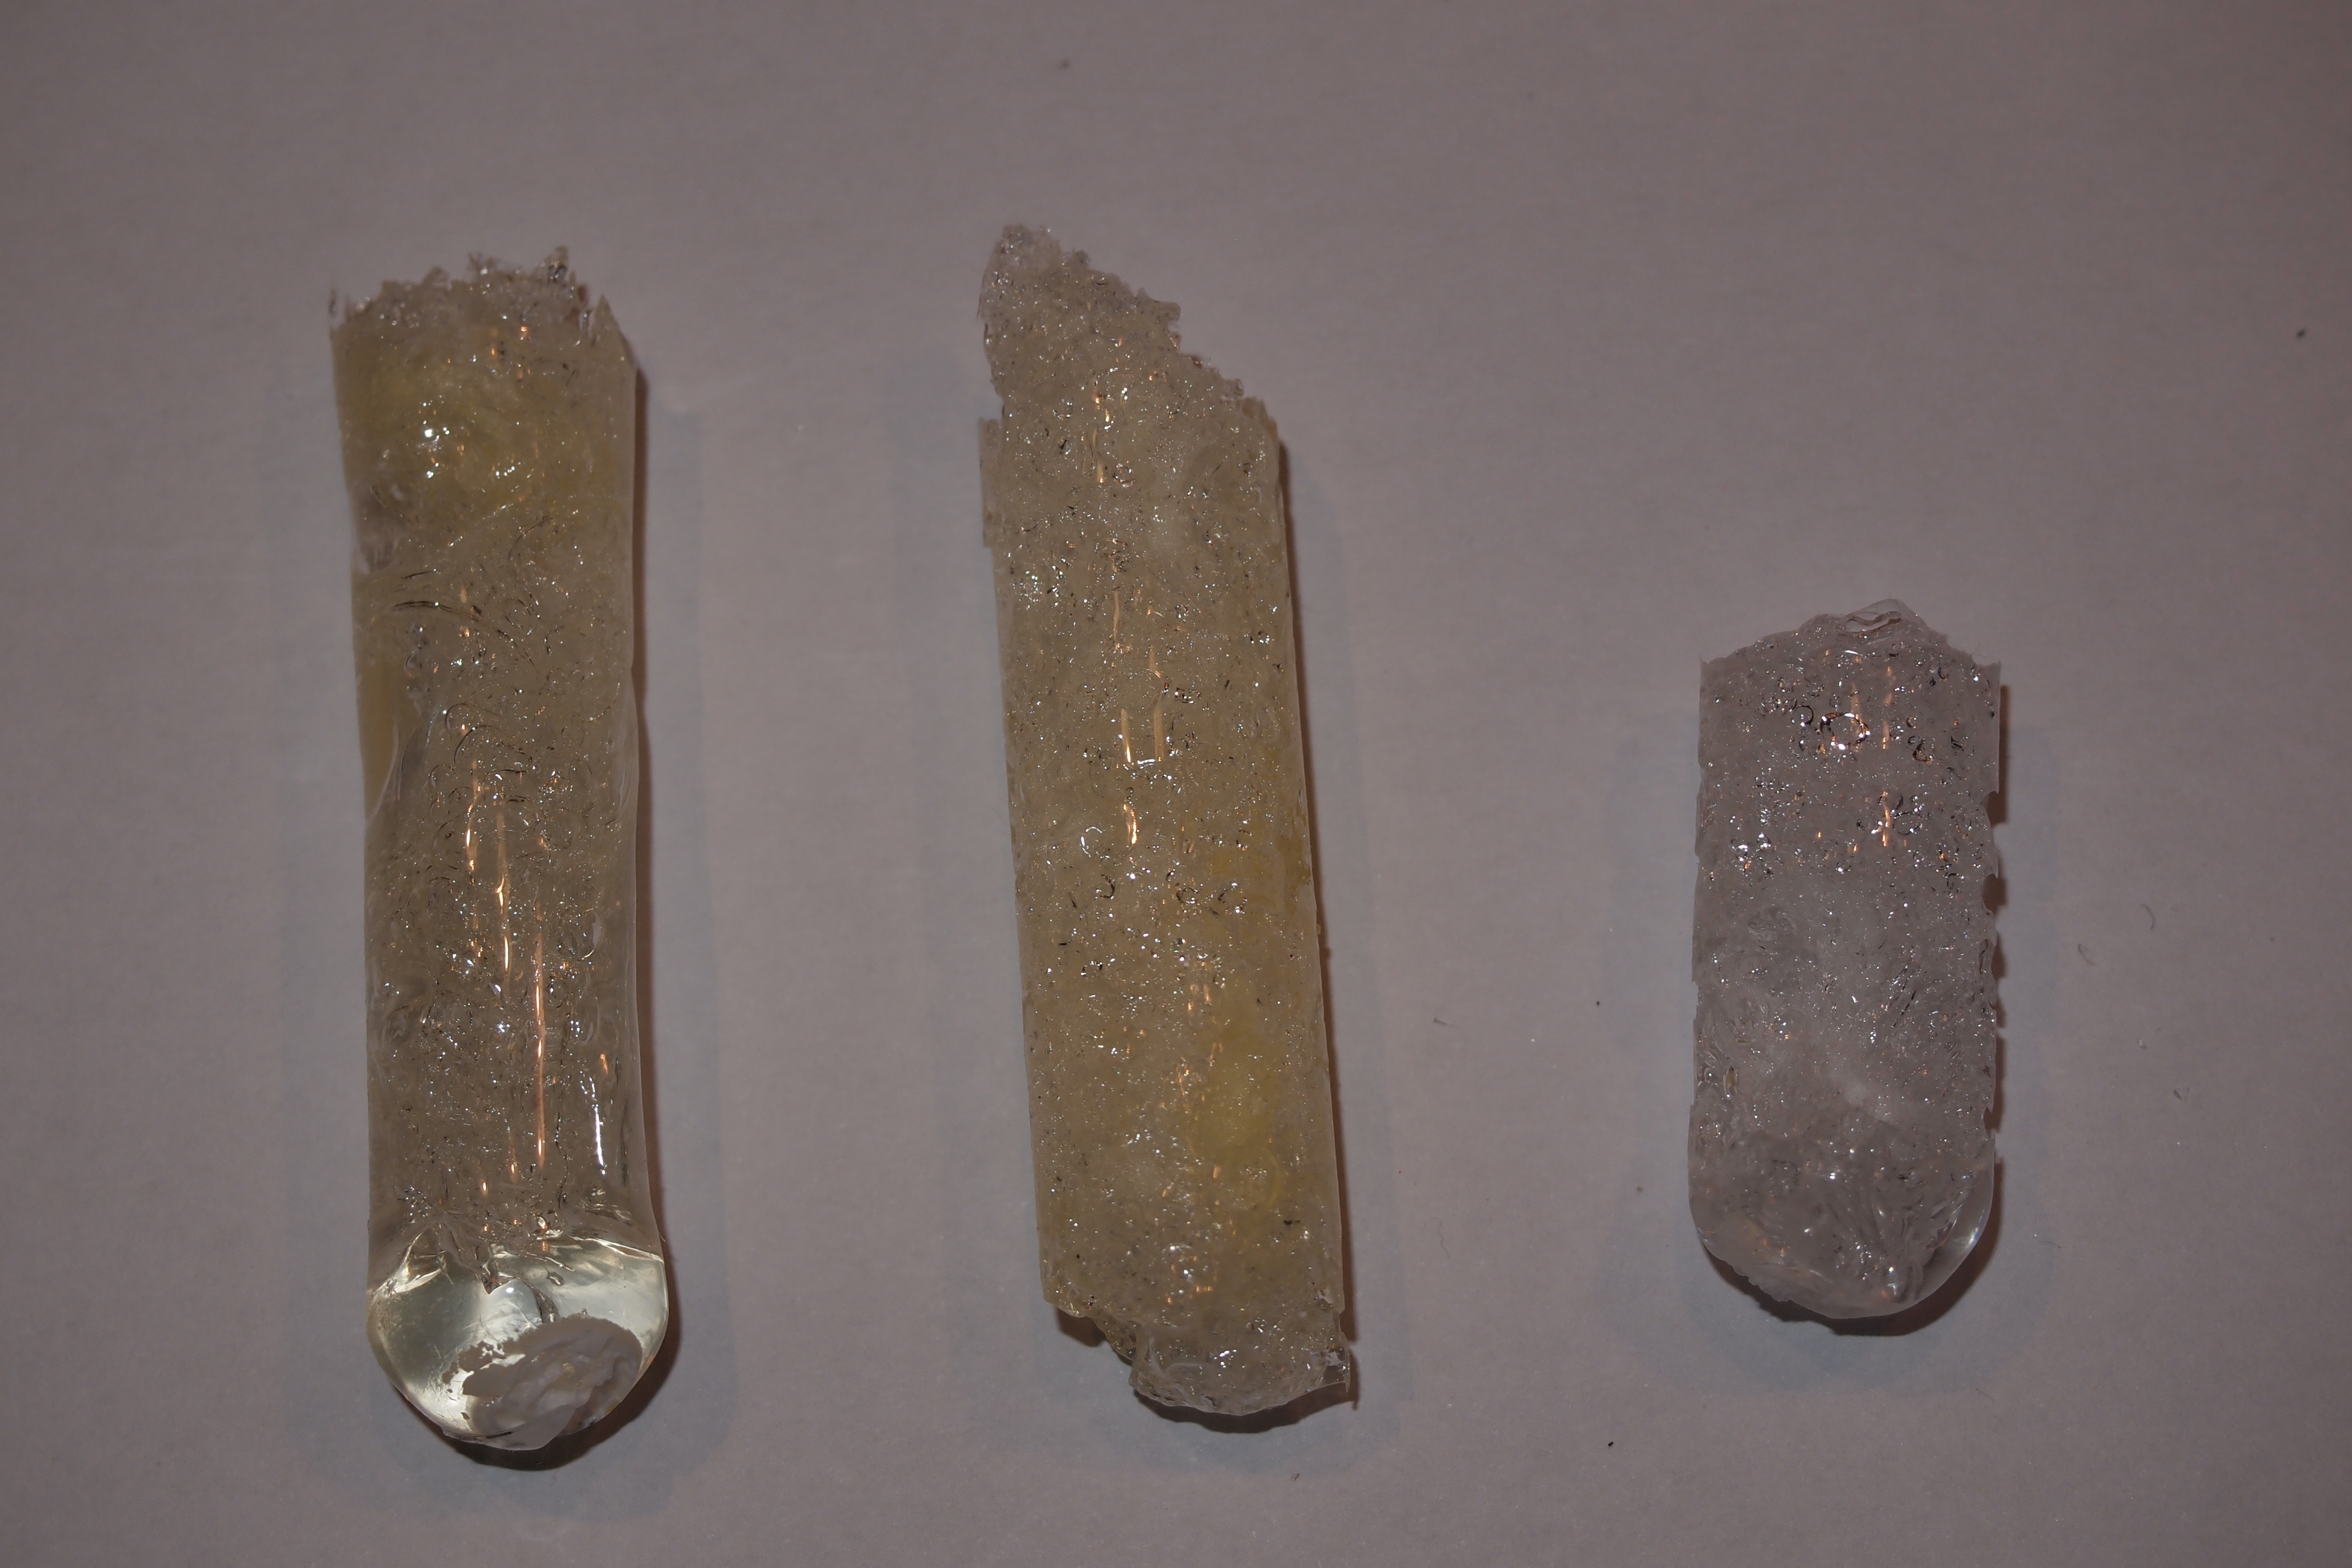
\includegraphics[height=0.1\textheight]{Bilder/Optische_Wellenleiter_Die_Polymer_Optische_Faser/Material_Polycarbonat/pmmastuecke.png}
                \caption[PMMA]{PMMA}
                \label{fig:cdquillt}
            \end{center}
        \end{minipage}
    \end{center}
\end{figure}

Ergebnis: Die entstandenen PMMA-Stücke haben eine geringe Qualität, da
Luftblasen in dem Kunststoff eingeschlossen sind, und eine gelbliche Färbung
erkennbar ist (unverbrauchtes AIBN). Jedoch lässt sich in kleinen Stücken die
hohe optische Durchlässigkeit von PMMA erkennen (siehe Abb. ...). Jedoch zeigt
der Versuch, dass man PMMA relativ einfach herstellen kann.

%TODO: Bild
